% !TEX program = lualatex

\documentclass{article}
\usepackage{luaotfload}
\usepackage{graphicx}
\usepackage{amsmath}

% load cmuntt here not from lua (for everyone except me, it seems)
\font\cmuntt = cmuntt at 12pt \cmuntt
\edef\cmunttid{\fontid\cmuntt}


\expandafter\let\expandafter\%\csname @percentchar\endcsname
\directlua {
 local cbl=luatexbase.callback_descriptions('define_font')
% print('\string\n======' .. cbl[1] .. '===\string\n')
original_fontloader=luatexbase.remove_from_callback('define_font',cbl[1])
luatexbase.add_to_callback('define_font',
function(name,size,i)
  if (name=='cmtt10x') then
% this works in my dev version but for older setups
% make sure cmuntt.otf has been loaded before we mess
% up the font loader.
%  f = original_fontloader('cmuntt.otf',size)
  f = font.getfont(\cmunttid)
              f.name = 'cmtt10x'
              f.type = 'virtual'
              f.fonts = {{ name = 'cmuntt', size = size}}
for j,v in pairs(f.characters) do
  local gr = 0.4*math.random()
  local gr2 = 0.4*math.random()
                       v.commands = {
{'lua','
  r1 = 0.01*math.random(-10,10)
pdf.print
(string.format(" q \%f \%f \%f \%f 0 0 cm ",
math.cos(r1), - math.sin(r1), math.sin(r1), math.cos(r1)
))'},
                           {'special','pdf: ' .. gr2 .. ' g'},
{'push'},
{'right', math.random(-20000,20000)},
{'down', math.random(-20000,20000)},
                           {'char',j},
{'pop'},
{'lua','pdf.print(" Q ")'},
{'down', math.random(-20000,20000)},
                           {'special','pdf: ' .. gr .. ' g'},
                           {'char',j},
                           {'special','pdf: 0 g'}

                         }
end
return f
else
return original_fontloader(name,size,i)
end
end,
'define font')
}

{\count0=0
\loop
\global\mathcode\count0=\count0
\ifnum\count0<256
\advance\count0 1
\repeat
}

\newcommand{\negphantom}[1]{\settowidth{\dimen0}{#1}\hspace*{-\dimen0}}

\def\sqrt#1{^^^^221a\overline{#1}}


\def\ph{\phantom}
\def\vph{\vphantom}
\def\hph{\hphantom}

\def\Hat#1{\hat{\vph{A}#1}}


\def\partial{\reflectbox{6}}
\def\nabla{\raisebox{\depth}{\scalebox{1}[-1]{Δ}}}
\def\={\; = \;}
\def\+{\; + \;}
\def\-{\; - \;}
\def\pm{\; ± \;}
\def\times{\; × \;}
\def\cdot{\; · \;}

\def\int{
  \raisebox{-\height}{J}
  \negphantom{J}
  \hspace{0.1em}
  I\negphantom{I}
  \hspace{0.1em}
  \raisebox{2\depth}{\scalebox{-1}[-1]{J}}
  \;
}

\def\oint{
  \hspace{0.1em}
  C
  \hspace{-0.4em}
  \raisebox{-\height}{J}
  \negphantom{J}
  \hspace{0.1em}
  I\negphantom{I}
  \hspace{0.1em}
  \raisebox{2\depth}{\scalebox{-1}[-1]{J}}
  \hspace{-0.4em}
  \reflectbox{C}
  \;\;
}

\renewcommand{\d}[1]{\;\const{d}#1}
\newcommand{\dd}[2]{\frac{\const{d} #1}{\const{d} #2} \;}
\newcommand{\pd}[2]{\frac{\partial  #1}{\partial  #2} \;}

\newcommand{\sub}[2]{
  \raisebox{0pt}[0pt][0pt]{#1\raisebox{-0.6ex}{#2}}
}


\begin{document}
$\relax$

\font\myfont= cmtt10x at 12pt \myfont
\font\myfonts= cmtt10x at 7pt
\let\selectfont\relax

\textfont0=\myfont
\scriptfont0=\myfonts 
\scriptscriptfont0=\myfonts 
\textfont1=\myfont
\textfont2=\myfont
\textfont3=\myfont


\centerline{Matematika pro fyziky 1: Riget}
\centerline{Mikkel Grnø}
\centerline{5. jan. 1992}


\section*{Překvapivý objev / 1. jan.}
Ano, přiznávám bez mučení, včera v noci jsem se vloupal do nemocnice. Ale než mě za takový lehkovážný čin odsoudíte, vyslechněte si nejdřív celý příběh. Popravdě je poněkud komické psát tímto tónem, když si tento dokument přečtu nanejvýš já a můj profesor z university, než jej spálím v krbu. Po tom, co jsem včera zažil, je ale netradiční volba vyprávěcího stylu asi ta nejméně bizarní věc.

Můj motiv byl prostý a pragmatický - před svátky mi v nemocnici Riget zemřela babička z matčiny strany a já, vědom si pochybné pověsti nemocnice, rozhodl jsem se vyšťárat na personál nějakou špínu. Nezdárně zakončené doktorské studium mě zanechalo bez peněz i bez práce a vidina nějakého finančního odškodnění za zesnulou příbuznou mě lákala. Využil jsem tedy novoroční vřavy, nepozorovaně rozbil okno v přízemí a vklouzl dovnitř.

Netrvalo mi dlouho proklouznout kolem noční směny v levém křídle - to nealkoholické šampaňské je asi zmohlo, proto všichni tři spokojeně podřimovali. Ani ne za deset minut jsem byl u dveří márnice. Zatímco doteď bylo všechno snadné popsat, správná slova pro to, co následovalo, se mi doteď nedaří najít. Při vzpomínce na včerejšek se mi stále ježí vlasy na zátylku, proto odpusťte, drahý prof. Ørstede, že se události ani nepokusím popsat, ale raději Vás na tuto prokletou půdu dovedu, abyste vše viděl na vlastní oči. Vězte ale, že má teorie - ta nemoderní, nefalsifikovatelná a paravědecká, kterou celý sbor, až na Vás, odsoudil - má teorie je správná!


\section*{Měření / 3. jan.}
Ubytoval jsem se v hotelu zhruba dva kilometry od nemocnice. Po dni shánění součástek, pájení a montování, podařilo se mi sestrojit eterický interferometr - první svého druhu. Dnes jsem se opět vloupal do nemocnice a provedl pečlivá několikahodinová měření. Má podezření se potvrdila: podařilo se mi naměřit uniformní vír v éteru. Prošel jsem s přístrojem všechna patra, o silné válcové symetrii není pochyb. Rychlostní pole víru lze popsat vzorcem:
\[
    v(r, φ, z) \= \frac{Γ}{2πr} \Hat{φ}.
\]
Osa $\Hat{z}$ se nachází asi 150 m severně od recepce nemocnice.

Protože při sobě bohužel nemám tabulky, budu si pro práci s válcovými souřadnicemi několik vztahů muset odvodit ručně. Válcové souřadnice jsou definovány:
\[ x \= r \cos φ \]
\[ y \= r \sin φ \]
\[ z \= z        \]
\\
Nyní si vyjádřím derivace polohového vektoru podle nových souřadnic:
\[
  R \= x\Hat{x} \+ y\Hat{y} \+ z\Hat{z}
\]
\[
  R \= r \cos φ \Hat{x} \+ r \sin φ \Hat{y} \+ z \Hat{z}
\]
\\
\[
  \sub{e}{r} \= \pd{R}{r} \= \ph{-r} \cos φ \Hat{x} \+ \ph{r} \sin φ \Hat{y}
\]
\[
  \sub{e}{φ} \= \pd{R}{φ} \= -r \sin φ \Hat{x} \+ r \cos φ \Hat{y}
\]
\[
  \sub{e}{z} \= \pd{R}{z} \= \Hat{z}
\]
\\
Velikosti těchto vektorů jsou Lamého koeficienty $\sub{h}{j} \= |\sub{e}{j}|$:
\[
  \sub{h}{r} \= \sqrt{ \cos^2 φ \+ \sin^2 φ } \= 1 \hph{r^2 r^2}
  \vph{\Bigg(}
\]
\[
  \sub{h}{φ} \= \sqrt{ -r^2 \sin^2 φ \+ r^2 \cos^2 φ } \= r
  \vph{\Bigg(}
\]
\[
  \sub{h}{z} \= 1 \hph{ \= \sqrt{ -r^2 \sin^2 φ \+ r^2 \cos^2 φ }}
  \vph{\Bigg(}
\]
\\
Bázové vektory jsou jednotkové vektory ve směru derivace $R$ podle dané souřadnice, tedy $\Hat{j} = \sub{e}{j} \; / \; \sub{h}{j}$:
\[
  \Hat{r} \= \ph{-}
  \cos φ \; \Hat{x} \+
  \sin φ \; \Hat{y}
  \vph{\Big(}
\]
\[
  \Hat{φ} \= -
  \sin φ \; \Hat{x} \+
  \cos φ \; \Hat{y}
  \vph{\Big(}
\]
\[
  \Hat{z} = \Hat{z}
  \vph{\Big(}
\]
\\
První dvě rovnice jsem vyřešil pro $\Hat{x}, \Hat{y}$:
\[
  \Hat{x} \= \cos φ \; \Hat{r} \- \sin φ \; \Hat{φ}
\]
\[
  \Hat{y} \= \sin φ \; \Hat{r} \+ \cos φ \; \Hat{φ}
\]
\\
Z řetízkového pravidla plynou vztahy mezi operátory parciálních derivací:
\[
  \pd{}{r} \= \pd{x}{r} \; \pd{}{x} \+ \pd{y}{r} \; \pd{}{y}
\]
\[
  \pd{}{φ} \= \pd{x}{φ} \; \pd{}{x} \+ \pd{y}{φ} \; \pd{}{y}
\]
\\
Vyřešením soustavy dvou rovnic a dosazením derivací jsem získal vztahy pro $\partial / \partial x$ a $\partial / \partial y$:
\[
  \pd{}{x} \= \cos φ \; \pd{}{r} \- \frac{1}{r} \sin φ \pd{}{φ}
\]
\[
  \pd{}{y} \= \sin φ \; \pd{}{r} \+ \frac{1}{r} \cos φ \pd{}{φ}
\]
\\
V kartézských souřadnicích vypadá operátor prostorové derivace takto:
\[
  \nabla \= \Hat{x}\pd{}{x} \+ \Hat{y}\pd{}{y} \+ \Hat{z}\pd{}{z}
\]
Za $\Hat{x}, \; \Hat{y}, \; \partial / \partial x$ a $\partial / \partial y$ můžeme dosadit. Po úpravě výrazu dostaneme:
\[
  \nabla \= \Hat{r}\pd{}{r} \+ \frac{1}{r}\;\Hat{φ}\pd{}{φ} \+ \Hat{z}\pd{}{z}
\]
Musím se přiznat, že si nepamatuji, že by odvození vzorce pro $\nabla$ v obecných orthogonálních souřadnicích bylo tak náročné - obzvlášť na psacím stroji mi trvalo zapsat postup několik hodin. Bohužel, peníze na nový počítač teď rozhodně nemám, budu to tedy muset nějak vydržet. Protože ale technicky vzato už je čtvrtého, pro dnešek toho bylo, myslím, víc než dost.

\section*{Pokračuji v měření / 4. jan.}
Měl bych být více obezřetný – kromě toho, že se mi dnes podařilo spálit interferometr, téměř mě objevil personál nemocnice. Tedy ne téměř – úplně. Naštěstí to ale byli jenom dva mentálně postižení umývači nádobí, kteří ani nepostřehli, že do nemocnice nepatřím.

Štěstí mně ale zatím přálo víc, než bych si troufal předpovídat. Nejenom, že jsem přes svou neopatrnost zůstal neodhalen, navíc jsem měl jednu z nejplodnějších fyzikálních diskusí svého života. Jeden z umývačů totiž, navzdory svým genetickým predispozicím, zřejmě rozumí fyzice na mnohem vyšší úrovni, než kdejaký akademik. A potvrdil mi mou teorii! Na území nemocnice se skutečně otevírá brána do duálního světa, což je jev, který je vždy doprovázen silným eterickým vírem. Nemůžu se dočkat, až budu zpět v nemocnici! Mezitím ale potřebuji vypracovat teoretický model, který mi o jevu řekne více.

Naštěstí i v této oblasti mi přál osud. V šuplíku pracovního stolu v mém hotelovém pokoji jsem objevil zápisky jistého P. Krtouše z roku 1984, kde bylo mj. odvození rotace pro obecné orthogonální souřadnice. Klíčové je použití Stokesova theorému.

\[
  \begin{array}{cccc}
    \int & \nabla \times a \cdot dS \= & \oint & a \cdot ds \\[2pt]
    S & & \partial S
  \end{array}
\]

\begin{figure}[h!]
  \centering
  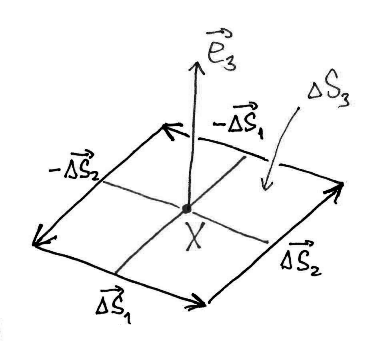
\includegraphics[width=0.6\textwidth]{krtous_element.png}
\end{figure}
Použijeme integraci na infinitesimálně malém čtverci o rozměru $Δs_1 \times Δs_2$, centrovaném v bodě $X$. Pro zkrácení zápisu jsem si zavedl body $X_{1+}, X_{1-}, X_{2+}, X_{2-}$, pro které platí:
\begin{align*}
  X_{j±} \= X \pm Δs_j
\end{align*}

Pro infinitesimální plošky a úsečky ze Stokesova theorému platí:

\begin{align*}
  \nabla \times a \cdot ΔS &\=
  a \cdot Δs \\
  \nabla \times a \cdot ( Δx^1 \times Δx^2 ) &\=
  a \cdot Δs_1(X_{2-}) + a \cdot Δs_2(X_{1-}) -
  a \cdot Δs_1(X_{2+}) - a \cdot Δs_2(X_{1+}) \\
  \nabla \times a \cdot h_1 h_2 ( Δξ^1 \times Δξ^2 ) &\=
  -Δs_2 \cdot \nabla (a^1 Δs_1) + Δs_1 \cdot \nabla (a^2 Δs_2) \\
  h_1 h_2 \nabla \times a \cdot ΔS' &\=
  Δξ^1 Δξ^2 ( - \pd{}{ξ^2}(a^1 h_1) + \pd{}{ξ^1}(a^2 h_2) )
\end{align*}

Složky rotace v obecných orthogonálních souřadnicích jsou tedy:
\begin{align*}
  \nabla \times a
  &\= \frac{1}{h_2 h_3}
  ( \pd{a^3 h_3}{ξ_2}-\pd{a^2 h_2}{ξ_3} ) \hat{ξ}_1 \\
  &\+ \frac{1}{h_3 h_1}
  ( \pd{a^1 h_1}{ξ_3}-\pd{a^3 h_3}{ξ_1} ) \hat{ξ}_2 \\
  &\+ \frac{1}{h_1 h_2}
  ( \pd{a^2 h_2}{ξ_1}-\pd{a^1 h_1}{ξ_2} ) \hat{ξ}_3
\end{align*}

Teď už jen dosadím Lamého koeficienty a máme vzorec pro rotaci ve válcových souřadnicích:
\begin{align*}
  \nabla \times a
  &\= \frac{1}{r}
  ( \pd{a_\text{z}}{φ}-\pd{a_\text{φ}}{z} ) \hat{r} \\
  &\+
  ( \pd{a_\text{r}}{z}-\pd{a_\text{z}}{r} ) \hat{φ} \\
  &\+ \frac{1}{r}
  ( \pd{r a_\text{φ}}{r}-\pd{a_\text{r}}{φ} ) \hat{z}
\end{align*}

Jediná nenulová derivace $v(r,φ,z)$ je $\partial v_\text{φ} / \partial r$, proto v rotaci pole zbude jenom jeden člen: 
\begin{align*}
  \nabla \times v
  &\= \frac{1}{r} ( \pd{}{r} r v_\text{φ} \- \pd{a_\text{r}}{φ} v_\text{φ} ) \hat{z} \\
  &\= \frac{1}{r} (\pd{}{r} r \frac{Γ}{2πr} \- \pd{a_\text{r}}{φ} 0 ) \hat{z} \\
  &\= \frac{1}{r} (\pd{}{r} \frac{Γ}{2π}) \hat{z} \\
  &\= \frac{1}{r} 0 \hat{z} \;\;\; \= \;\;\; 0.
\end{align*}
Vidíme, že rotace je nulová. Mezitím pro cirkulaci kolem osy víru platí:
\[
  \begin{array}{cccc}
    & & 2π \\[2pt]
    \oint & v \cdot ds \=
    & \int & v(R,φ,0) \cdot \hat{φ} \; R dφ \= \\[2pt]
    c & & 0
  \end{array}
\]
\[
  \begin{array}{cccc}
    & 2π \\[5pt]
    \= & \int & \dfrac{Γ}{2πR} R \; dφ \;\; \= \;\; Γ. \\[5pt]
    & 0
  \end{array}
\]
Vidíme, že rotace a cirkulace nesplňují Stokesův theorém – to je zjevně způsobeno singularitou ve středu eterického víru. Tato eterická singularita je elementárním pojítkem mezi dvěma světy, a jak vyplývá z teorie blíže diskutované v mé doktorské práci, jedinně v případě, kdy se eterické a anti-eterické excitace přesně vyruší a $\nabla \times v \= 0$, tehdy je pro člověka bezpečné mezi světy projít. Z naměřené hodnoty $Γ$ usuzuji, že bude vír stabilní řádově po dobu desítek hodin, proto nesmím promarnit šanci. Zítra vyhledám střed víru a jako první člověk se ocitnu zcela mimo náš časoprostor. Nemohu se dočkat, co mě čeká! Hned po návratu podám další informace!

\pagebreak

\section*{Návrat / 5. jan.}


\end{document}
